\documentclass[convert={density=300,outext=.png}]{standalone}
\usepackage{tikz}
\usetikzlibrary{backgrounds}

\begin{document}
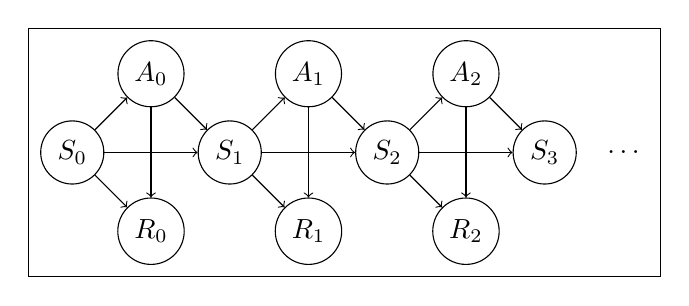
\begin{tikzpicture}[framed]

  \node[circle,draw] at (0,0) (S0) {$S_0$};
  \node[circle,draw] at (1,1) (A0) {$A_0$};
  \node[circle,draw] at (1,-1) (R0) {$R_0$};
  
  \node[circle,draw] at (2,0) (S1) {$S_1$};
  \node[circle,draw] at (3,1) (A1) {$A_1$};
  \node[circle,draw] at (3,-1) (R1) {$R_1$};
  
  \node[circle,draw] at (4,0) (S2) {$S_2$};
  \node[circle,draw] at (5,1) (A2) {$A_2$};
  \node[circle,draw] at (5,-1) (R2) {$R_2$};
  
  \node[circle,draw] at (6,0) (S3) {$S_3$};
  \node at (7,0) (dots) {$\dots$};
  
  \draw[->] (S0)--(A0);
  \draw[->] (S0)--(S1);
  \draw[->] (S0)--(R0);
  \draw[->] (A0)--(R0);
  \draw[->] (A0)--(S1);
  
  \draw[->] (S1)--(A1);
  \draw[->] (S1)--(S2);
  \draw[->] (S1)--(R1);
  \draw[->] (A1)--(R1);
  \draw[->] (A1)--(S2);
  
  \draw[->] (S2)--(A2);
  \draw[->] (S2)--(S3);
  \draw[->] (S2)--(R2);
  \draw[->] (A2)--(R2);
  \draw[->] (A2)--(S3);
  
\end{tikzpicture}
\end{document}
